%!TEX root = ../research_proposal.tex

\section{BUMPER - Bug Meta-repository For Developers \& Researchers\label{sec:BUMPER}}

With the goal to support the research towards analyzing relationships between bugs and their fixes we constructed a dataset of 380 projects, more than 100,000 resolved/fixed and with 60,000 changesets that were involved in fixing them from Netbeans and The Apache Software foundation’s software that is (1) searchable in natural language at research.mathieu-nayrolles.com/bumper, (2) contains clear relationships between the bug report and the code involved to fix it, (3) supports complex queries such as parent-child relationships, unions or disjunctions and (4) provide easy exports in json, csv and xml format.

In what follows, we will present the projects we selected. Then, we present the features related to the bugs and their fixes we integrate in BUMPER (BUg Metarepository for dEvelopers and Researchers) and how we construct our dataset. Then, we present the API, based on Apache Solr \cite{Nayrolles2014b}, which allows the NLP search with practical examples before providing research opportunities based on our dataset.


However, to the best of our knowledge, no attempt have been made towards building an unified and online dataset where all the information related to a bug, or a fix can be easily accessed by researchers and engineers.

\subsection{Data collection}


Figure \ref{fig:bumper-approach} illustrates our data collection and analysis process that we present here and discuss in more detail in the following subsections. First, we extract the raw data from the two bug report management systems used in this study (Bugzilla\footnote{https://netbeans.org/bugzilla/} and Jira\footnote{https://issues.apache.org/jira/issues/?jql=}). The extracted data is consolidated in one database called BUMPER where we associate each bug report with its fix. The fixes are mined from different type of source versioning system. Indeed, Netbeans is based on mercurial\footnote{ http://mercurial.selenic.com/} while we used the git\footnote{http://git-scm.com/} mirrors\footnote{https://github.com/apache} for the Apache Foundation software.

\begin{figure}[h!]
  \centering
    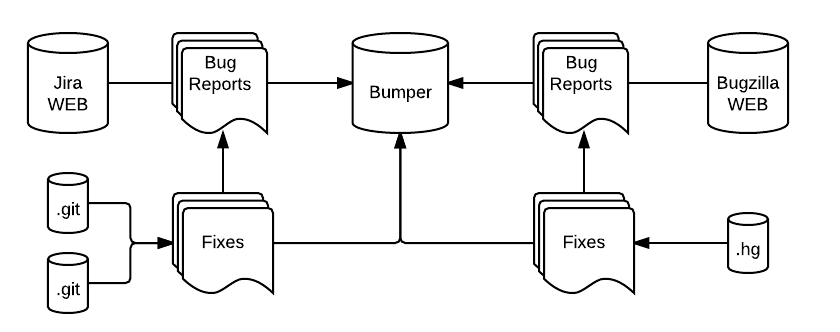
\includegraphics{media/bumper-approach.png}
    \caption{Overview of the bumper database construction.
    \label{fig:bumper-approach}}
\end{figure}

We used the same datasets presented earlier in Table \ref{table:datasets}.
We choose to use the same ones as these two datasets because they exposed a great diversity in programming languages, teams, localization, utility and maturity. Moreover, the used different tools, i.e. Bugzilla, JIRA, Git and Mercurial, and therefore, BUMPER is ready to host any other datasets that used any composition of these tools.

\subsection{Architecture}

{\tt BUMPER} rely on a highly scalable architecture composed of two distinct servers as depicted in Figure \ref{fig:bumper-arch}. The first server, on the left, handle the web requests and runs three distinct components:

\begin{itemize}
	\item Pound is a lightweight open source reverse proxy program and application firewall.
	It also serve us to decode https to request to http. Translating an https request to http and then, use this http request insteaad of the https one allow us to save the https decryption time required on each step.
	Pound also acts as a load-balancing service for the lower levels.
	\item Translated requests are then handle to Varnish. Varnish is an http accelerator designed for content-heavy and dynamic websites. What it does is caching request that come in and serve the answer from the cache is the cache is still valid.
	\item NginX (pronounced engine-x) is a web-server that has been developed with a particular focus on high concurrency, high performances and low memory usage.
\end{itemize}

On the second server, that concretely handle our data, we have the following items:

\begin{itemize}
	\item Pound. Once again, we use pound here, for the exact same reasons.
	\item SolrCloud is the scalable version of Apache Solr where the data can be separated into shards (e.g chunk of manageable size). Each shard can be hosted on a different server but its still indexed in a central repository. Hence, we can guarantee a low query time while exponentially increasing the data.
	\item Lucene is the full text search engine powering Solr. Each Solr server have its own embedded engine.
\end{itemize}

\begin{figure}[h!]
  \centering
    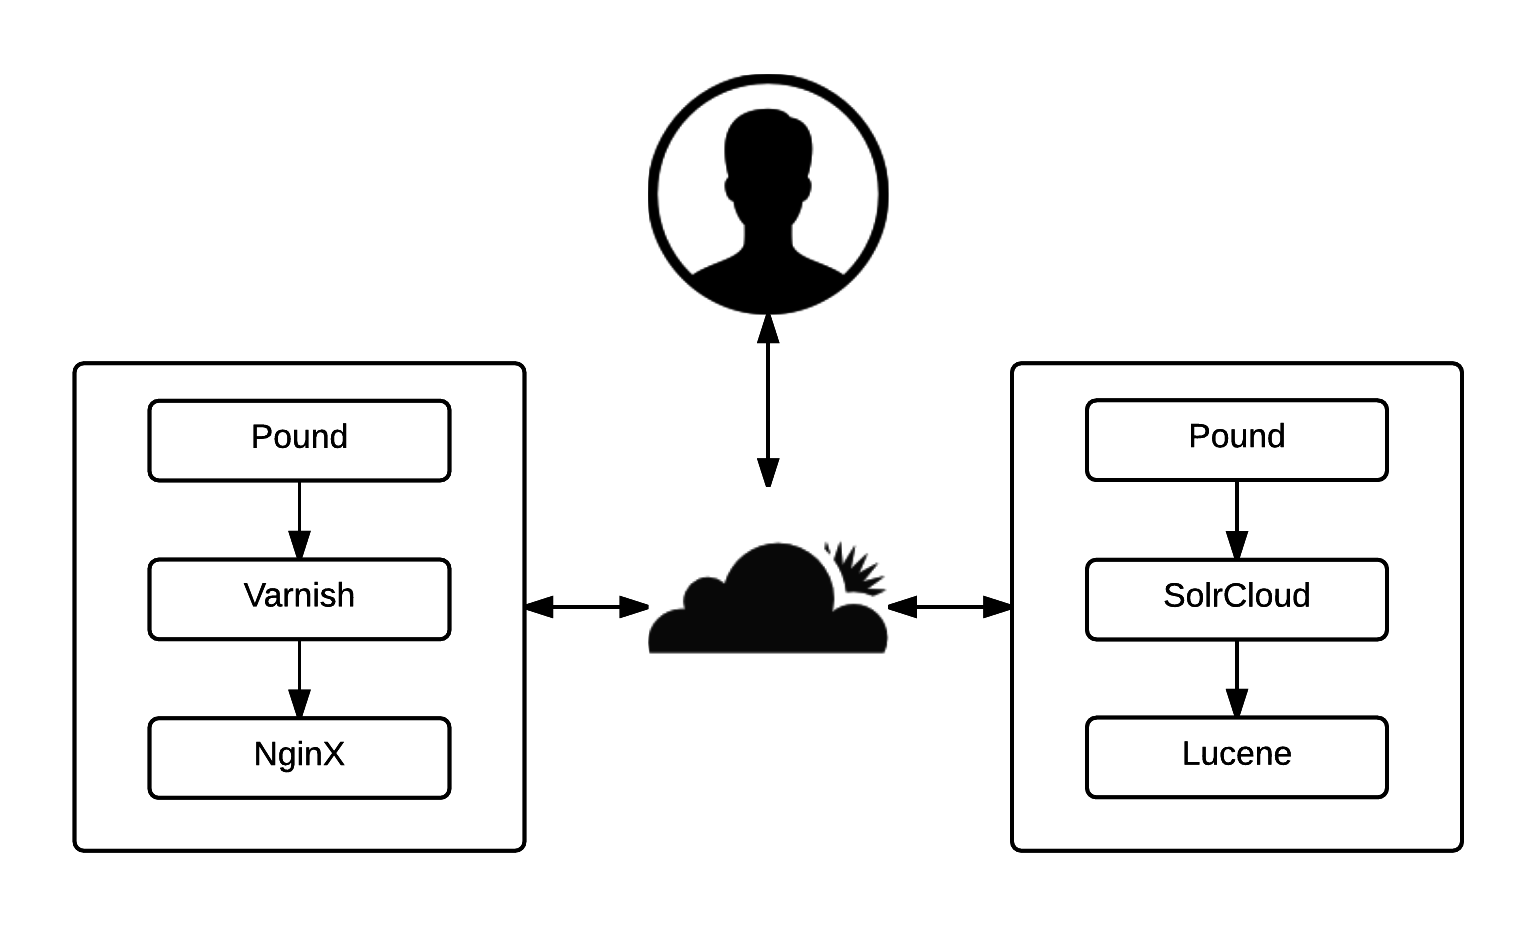
\includegraphics{media/bumper-arch.png}
    \caption{Overview of the bumper architecture.
    \label{fig:bumper-arch}}
\end{figure}

Request from users to the servers and the communication between our servers are going through the CloudFlare network.
CloudFlare acts as a content delivery network sitting between the users and the webserver.
They also provide an extra level of caching and security.

To give the reader a glimpse about the performances that this unusual architecture can yield; we are able to request and display the result of a specific request in less than 100 ms while our two servers are, in fact, two virtual machines sharing an AMD Opteron(tm) Processor 6386 SE (1 core @ 2,000 MHz) and 1 Gb of RAM.

\subsection{UML Metamodel}

Figure \ref{fig:bumper-approach} presents the simplified {\tt BUMPER} metamodel that we designed according to our bug taxonomy presented in section \ref{fig:bug-taxo} and according to our future needs for {\tt JCHARMING}, {\tt RESSEMBLE} and {\tt BIANCA}.

\begin{figure}[h!]
  \centering
    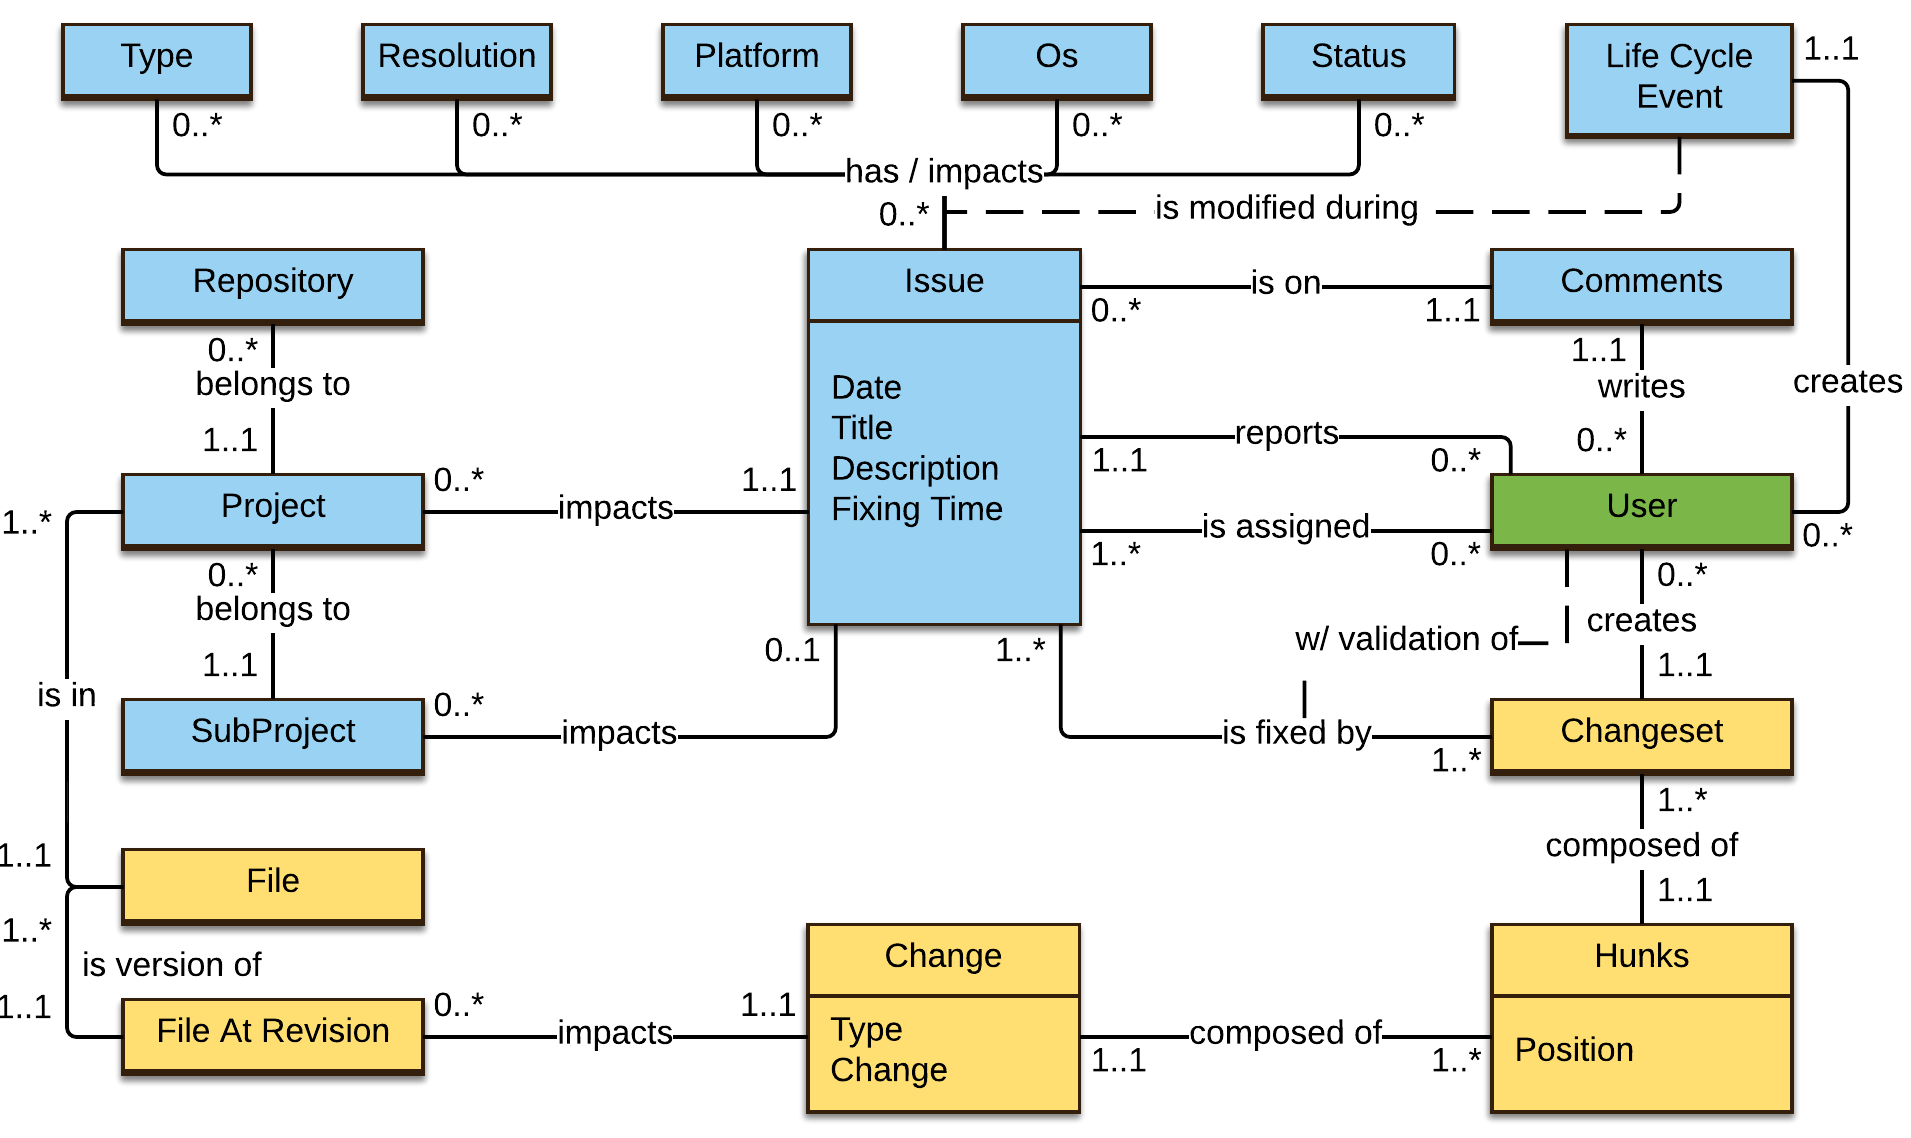
\includegraphics{media/bumper-model.png}
    \caption{Overview of the bumper meta-model.
    \label{fig:bumper-approach} }
\end{figure}


An {\it issue} ({\it task}) is characterized by a {\it date}, {\it title}, {\it description}, and a {\it fixing time}. They are reported (created) by and assigned to {\it users}.
Also, {\it issues} ({\it tasks}) belong to {\it project} that are in {\it repository} and might be composed of {\it sub-projects}.
{\it Users} can modify an {\it issue } ({\it task})  during {\it life cycle events} which impact the {\it type}, the {\it resolution}, the {\it platform}, the {\it OS} and the {\it status}. {\it Issues} ({\it tasks}) are resolved (implemented) by {\it changeset} that are composed of {\it hunks}. {\it Hunks} contain the actual changes to a {\it file} at a given revision which are version of the {\it file} entity that belongs to a {\it Project}.


\subsection{Features}

In this section, we present the features of bug report and their fixes in details.

\subsubsection{Bug Report}

A bug report is characterized by the following features:


\begin{itemize}

\item ID: unique string id of the form bug\_dataset\_project\_bug\_id
\item Dataset: the dataset of which the bug is extracted from.
\item Type: The type help us to distinguish different type of entities in BUMPER, i.e the bugs, changesets and hunks. For bug report, the type is always set to BUG
\item Date: The date at which the bug report has been submitted.
\item Title: The title of the bug report.
\item Project: The project that this bug affects.
\item Sub\_project: The sub-project that this bug affects.
\item Full\_name\_project: The combination of the project and the sub-project.
\item Version: the version of the project that this bug affects
\item Impacted\_platform: the platform that this bug affects
\item Impacted\_os: the operating system that this bug affects
\item Bug\_status: The status of the bug. As in bumper, our main concern is on the relationship between of fix and a bug, we only have RESOLVED bugs
\item Resolution: How the bug was resolved. Once again, as we are interested in investigating the fixes and the bugs, we only have FIXED bugs.
\item Reporter\_pseudo: the pseudonym of the person who report the bug.
\item Reporter\_name: the name of the person who reported the bug
\item Assigned\_to\_pseudo: the pseudonym of the person who have \item been assigned to fix this bug
\item Assigned\_to\_name: the name of the person who have been assigned to fix this bug
\item Bug\_severity: the severity of a bug
\item Description: the description of the bug the reporter gave
\item Fixing\_time: The time it took to fix the bug, i.e the elapsed time between the creation of the BR and its modification to resolved/fixed, in minutes
\item Comment\_nb: How many comments have been posted on the bug report system for that bug
\item Comment: Contains one comment. A bug can have 0 or many comments
\item File: A file qualified name that have been modified in order to fix a bug. A bug can have 0 (in case we did not find its related commit) or many files.

\end{itemize}

We selected these set of features for bug report as they are the ones that are analyzed in many past and recent studies. In addition, bugs can contains 0 or many changesets.

\subsubsection{Changesets}

In this sections, we present the features that characterize changeset entities in BUMPER.

\begin{itemize}

\item ID: the SHA1 hash
\item User: the name and email of the person who submitted that commit
\item Date: the date at which this commit has been fixed
\item Summary: the commit message entered by the user
\item File: The fully qualified name of a file modified on that commit. A changeset can have 1 or many files.
\item Number\_files: How many files have been modified in that commit
\item Insertions: the number of inserted lines
\item Deletions: the number of deleted lines
\item Churns: the number of modified lines
\item Hunks: the number of set of consecutive changed lines
\item Parent\_bug: the id of the bug this changeset belong to.

\end{itemize}

In addition, changesets contain one or many hunks.

\subsubsection{Hunks}
A hunks is a set of consecutive lines changed in a file in order. A set of hunks form a fix that can be scattered across one or many files. Knowing how many hunks a fixed required and what are the changes in each of them is useful, as explained by [2] to understand how many places developers have to go to fix a bug.

Hunks are composed of:

\begin{itemize}
\item ID: unique id based on the files, the insertion and the SHA1 of the commit
\item Parent\_changeset: the SHA1 of the changeset this hunks belong to
\item Parent\_bug: the id of the bug this hunk belongs to.
\item Negative\_churns: how many lines have been removed in that hunks
\item Positive\_churns: how many lines have been added in that hunks
\item Insertion: the position in a file at which this hunk takes place.
\item Change: One line that have been added or removed. A Hunk can contains one or many changes.
\end{itemize}

\subsection{Application Program Interface (API)\label{sec:bumper-api}}

BUMPER is available for engineers and researchers at {\bf https://bumper-app.com} and take the form of a regular search engine. Bumper supports (1) natural language query, (2) parent-child relationships query, (3) disjunctions and union between complex queries and (4) a straight forward export of queries results in XML, CSV or JSON format.

Browsing BUMPER, the basic query mode perform the following operation:

\begin{equation}
\begin{split}
(type:BUG~AND~report\_t:(``YOUR~TERMS''))~OR~(!parent~which=type``BUG'')~\\fix\_t:``YOUR~TERMS'')
\end{split}
\end{equation}

The first part of the query component of the query retrieve all the bugs that contains the $``YOUR~TERMS''$ query in at least one its features by selecting type:BUG and report\_t, which is an index composed of all the features of the bug, set to $``YOUR~TERMS''$.
Then, we merge this query with another one that reads \\
$(!parent~which=type``BUG'')fix\_t:~``YOUR~TERMS'')$.
In this one, we retrieve the parent documents, i.e the bugs, of fixes that contains $``YOUR~TERMS''$ in their $fix\_t$ index.
The $fix\_t$ index is, as for the BUG, an index based on all the field of changeset and hunk both. As a result, we search seamlessly in bugs report and their fixes in natural language.

As a more practicle example, Figure \ref{fig:bumper-live} illustrate a query on https://bumper-app.com. The search term is  ``{\it Exception}'' and we can see that 20,285 issues / tasks have been found in 25 ms. This particular set of issues, displayed on the left side, match because they contain ``{\it Exception}'' in the issue report or in the source code modified to fix this issue (implement this task). Then on the right side of the screen, the selected issue (task) is displayed. We can see the basic characteristic of the issue (task) followed by comments and finally, the source code.

\begin{figure}[h!]
  \centering
    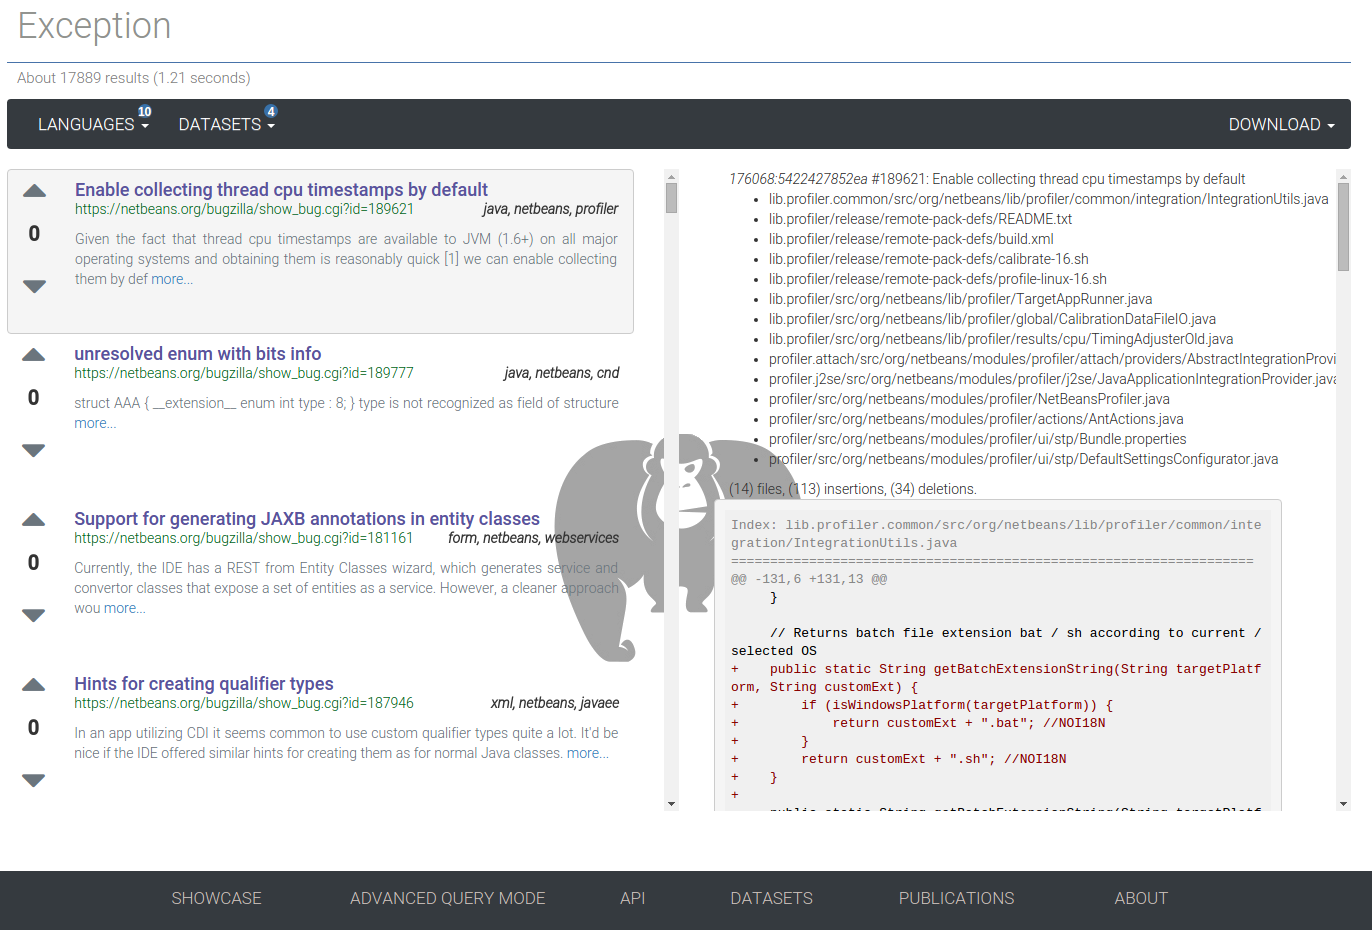
\includegraphics[scale=0.4]{media/bumper-live.png}
    \caption{Screenshot of https://bumper-app.com with ``Exception'' as research.
    \label{fig:bumper-live}}
\end{figure}


Moreover, BUMPER supports AND, OR, NOR operators and provide results in order of seconds.

As we said before, BUMPER is based on Apache Solr which have an incredibly rich API that is available online\footnote{ http://lucene.apache.org/solr/resources.html}.

{\tt BUMPER} serves as data repositories for the upcoming approaches presented in the next sections.
